\section{ALGORITHM}

The objective of this algorithm is to rapidly determine a feasible, time-optimal trajectory under uncertain goal constraints. 
Our focus is on drone interception scenarios, where a defense drone must intercept a target drone flying in the same cluttered environment. 
The position of the target drone is uncertain and must be determined using a prediction model. 
We account for the realistic scenario where predictions are imperfect and time-varying, requiring rapid adaptation of the defense drone's trajectory based on the target drone’s movements.

We assume that the distribution of goal positions is obtained from the prediction model, and candidate target positions are sampled from this distribution. 
Specifically, goal candidates $[\tilde p_{\text{goal}}^1, T_{\text{goal}}^1], \dots, [\tilde p_{\text{goal}}^K, T_{\text{goal}}^K]$ are selected considering both position and arrival time.
Based on these predictions of the target drone's position, we formulate the optimization of the defense drone's trajectory $p$ as follows:

\begin{equation}
\begin{aligned}
&\underset{p, k}{\text{minimize}} \; T_{\text{goal}}^k \;\;\; \text{subject to}\\
&p(T_{\text{goal}}^k) = \tilde p_{\text{goal}}^k, \; p(0) = \tilde p_{\text{init}},\; \mathcal{D\,} p(0) = \mathcal{D\,} \tilde p_{\text{init}}, \\
&p \in \mathcal{P}(\mathcal{D\,} \tilde p_{\text{init}}),\; p \in \mathcal{F}
\label{eqn:planning_homotopy}
\end{aligned}
\end{equation}

% $\tilde{p}_{\text{init}}$ and $\mathcal{D\,} \tilde p_{\text{init}}$ are respectively the current reference position and the current reference flat output state, which are derived from the previous reference trajectory. 
% $\mathcal{P}(\mathcal{D\,} \tilde p_{\text{init}})$ represents the set of feasible trajectories starting from the state $\mathcal{D\,} \tilde p_{\text{init}}$, $\mathcal{F}$ is the set of non-colliding trajectories.

% We employ a minimum-snap trajectory formulation that uniquely determines the polynomial representation based on a sequence of waypoints and the time allocated between them. 
% Unlike typical minimum-snap trajectory optimization problems, our proposed algorithm co-optimizes the waypoints and their time allocations. 
% The shortest path toward each goal candidate is initially found using A* search without considering the dynamics model. 
% From each A* path candidate, sequences of waypoints are sampled using the knot optimization method. 
% Subsequently, time allocations for all waypoint sequences are determined in parallel using the planning policy. 
% This policy not only provides time allocations but also assesses feasibility. 
% Finally, we select the feasible trajectory with the minimum traversal time as the defense drone's trajectory.

% \cref{fig:alg_overview} outlines our proposed algorithm. 
Our proposed algorithm consists of the following steps:
First, we use A* search to find the shortest path to each goal candidate generated by the target position prediction model. 
From these paths, we sample waypoint sequences using knot optimization. 
Next, our planning policy simultaneously determines time allocations for all sequences and assesses their reachability. 
Lastly, we select the reachable trajectory with the minimum traversal time for the defense drone.

\subsection{Waypoints candidates selection}

% We determine the path towards the target position using A* search on the available occupancy map. 
% The heuristic used in the A* search is directed towards the center of the goal candidates’ points, and the search continues until it reaches all candidates. 
% To enhance the computation speed of the search, we employ a multi-resolution occupancy map as shown in Figure \ref{fig:multi_resol_astar}.
% The original high-resolution map is downsampled using max pooling, and the grid resolution is dynamically adjusted based on the distance between the defense drone and the target drone at the current time step. 
% Specifically, a lower resolution map is employed when the drones are farther apart. 
% The default lattice size starts at 0.1 m. 
% As the distance between the target and defense drones exceeds 10\%, 20\%, and 40\% of the diagonal size of the target environment's room, the lattice size of the A* search grid increases to 0.2 m, 0.5 m, and 1 m, respectively.
We use A* search on a multi-resolution occupancy map to determine the path to the target. 
The heuristic is directed towards the center of goal candidates' points, continuing until all candidates are reached. 
To speed up computation, we employ a dynamically adjusted grid resolution based on the distance between drones. 
The default lattice size is 0.1 m, increasing to 0.2 m, 0.5 m, and 1 m as the inter-drone distance exceeds 10 \%, 20 \%, and 40 \% of the room's diagonal, respectively, as shown in \cref{fig:multi_resol_astar}.

\begin{figure}[]
    \centering
    % \captionsetup{justification=centering}
    \includegraphics[width=0.48\textwidth,trim=0.15cm 2.8cm 0.15cm 1.5cm,clip]{figures/multi_resol_astar.png}
    \caption{Utilizing a multi-resolution occupancy map for efficient A* search, where the lattice size increases with the distance between the target and defense drones.}
    \label{fig:multi_resol_astar}
    \vspace{-2.0\baselineskip}
\end{figure}

% Initially, we select waypoints along the A* path to generate a trajectory that fully incorporates the dynamics model of the vehicle. 
% These waypoints are then reconnected using the minimum snap method, aligning the optimized trajectory closely with the initial A* path. 
% We employ the knot optimization technique, commonly used in computer-aided design (CAD) and geometric modeling, where piecewise continuous polynomials help construct regression models from data or simplify high-dimensional simulation results. 
% The main challenge is selecting appropriate knot points—the endpoints of these polynomial segments—to minimize the error between the model and the actual data. 
% Several methods have been proposed for selecting knot points based on parameterizations of the data’s derivatives~\cite{yeh2020fast} or curvature~\cite{hernandez2003sampling}.
% We adopt a combination of distance and curvature parameterizations, as outlined in \cite{pagani2018curvature}.

We select waypoints along the A* path to generate a trajectory incorporating the vehicle's dynamics model. 
These waypoints are reconnected using the minimum snap method~\cite{yeh2020fast, hernandez2003sampling}, aligning the optimized trajectory with the initial path. 
We use knot optimization, a technique from Computer-Aided Design and geometric modeling, to select appropriate endpoints for polynomial segments. Our approach combines distance and curvature parameterizations as described by \cite{pagani2018curvature}. 
To elaborate, the initial A* path $\tilde{\mathbf{q}} = [\tilde{q}^1 \cdots \tilde{q}^M]$ is reparameterized as follows:
\begin{align}
k_{d} (s) &= {\sum \nolimits}_{i=1}^{s} d(\tilde{q}^{i-1}, \tilde{q}^{i}) \\
k_{c} (s) &= {\sum \nolimits}_{i=1}^{s-1} R(\tilde{q}^{i-1}, \tilde{q}^{i}, \tilde{q}^{i+1})^{-1} (k_{d}(s+2) - k_{d}(s)) / 2 \\
k(s) &= (k_d(s) + k_c(s)) / 2
\end{align}
where $d(\cdot)$ is the Euclidean distance between adjacent points, and $R(\cdot)$ is the radius of the circle through three consecutive points.
Along the parameterization $k(s)$, we uniformly select $N_\text{wps}$ waypoints ($\tilde{\mathbf{p}} = [\tilde p^1 \cdots \tilde p^{N_\text{wps}}]$) along the A* path. 
The number of waypoints is determined as:
\begin{align}
N_{\text{wps}} = \max (k_{d}(M) / k_{d, \text{min}}, k_{c}(M) / k_{c, \text{min}})
\end{align}
where $k_{d}(M)$ and $k_{c}(M)$ represent a total distance and curvature.
$k_{d, \text{min}}$ and $k_{c, \text{min}}$ are tunable hyperparameters. 
The number of waypoints is constrained by the minimum and maximum lengths of the waypoints sequence used for training the policy, which are 2 and 14, respectively.


\subsection{Iterative traversal time adaptation}
% The planning policy determines the time allocations between sequences of remaining waypoints. 
% It is based on a sequence-to-sequence language model, trained to output the minimum time allocation from an input consisting of a waypoints sequence and initial state. 
% The outputs from the planning policy are then used to generate a polynomial trajectory using quadratic programming in the minimum snap method. 
% We compare two different policy models: one trained with the fastest minimum snap trajectory using supervised learning (Pretrained), and another refined further with reinforcement learning (MFRL).

% We propose an iterative traversal time adaptation method to adjust the output trajectory so that it reaches the target points simultaneously with the arrival time. 
% In drone interception scenarios, it is advantageous to arrive at the final points simultaneously rather than moving as fast as possible and then waiting. 
% Since the target positions are uncertain and time-varying, approaching as slowly as possible maintains more planning options, while moving at the fastest speed may be less effective because it limits the ability to change direction easily.

The planning policy outputs minimum time allocations for waypoint sequences, used to generate polynomial trajectories via QP in \eqref{eqn:minsnap_1}. 
As this policy only produces minimum-time trajectories, we propose an iterative traversal time adaptation method to adjust for simultaneous arrival with the target. 
In drone interception, this approach is preferable to maximum speed, maintaining more planning options given uncertain, time-varying target positions and allowing easier direction changes.

We leverage the property that the shape of the minimum snap trajectory remains invariant when both time allocation and the current trajectory state are scaled.
To be specific, the polynomial $\chi(\alpha \mathbf{x}, \tilde {\mathbf{p}}, \alpha^{-1}\mathcal{D\,} \tilde p)$ maintains a consistent shape across all scale factors $\alpha\in\mathbb{R}_{>0}$ where $\alpha^{-1}\mathcal{D\,} \tilde p$ is defined as
\begin{equation}
\alpha^{-1} \mathcal{D\,} \tilde p \coloneqq 
\begin{bmatrix}
\alpha^{-1} \tilde{p}_r^{(1)} \kern2pt \cdots \kern2pt \alpha^{-4} \tilde{p}_r^{(4)} \kern2pt \alpha^{-1} \tilde{p}_\psi^{(1)} \kern2pt \alpha^{-2} \tilde{p}_\psi^{(2)}
\end{bmatrix}.
\label{alg:scale_property}
\end{equation}
When $\alpha > 1$, this transformation slows the trajectory while preserving its shape.

As illustrated in \cref{fig:diagram_iter}, we propose a scaling method based on this property.
%%%%%%%%%%%%%%%%%%%%%%%%%%
We generate scaled time allocations using the planning policy $\pi$ as follows:
\begin{equation}
    \mathbf{x} = \alpha \pi (\tilde{\mathbf{p}}, \alpha \mathcal{D\,} \tilde p)
\end{equation}
where $\alpha > 1$ speeds up the initial trajectory state $\mathcal{D\,} \tilde p$ and slows down the policy output.
This scaling method is derived by considering that the policy generates a feasible trajectory $\chi(\pi (\tilde{\mathbf{p}}, \alpha \mathcal{D\,} \tilde p), \tilde {\mathbf{p}}, \alpha \mathcal{D\,} \tilde p)$ for the initial state with $\alpha > 1$, which, when applying the scaling transformation \eqref{alg:scale_property}, yields $\chi(\alpha \pi (\tilde{\mathbf{p}}, \alpha \mathcal{D\,} \tilde p), \tilde {\mathbf{p}}, \mathcal{D\,} \tilde p)$, resulting in the same-shaped time allocations for the original initial state.
In practice, speeding up the initial state produces a more conservative policy output, which, when scaled back down, results in final time allocations that are still slower than those without scaling, reducing tracking error as shown in \cref{fig:scale_factor_err}.
%%%%%%%%%%%%%%%%%%%%%%%%%% 
% We initially scale the trajectory state by \llbcomment{multiplying the scale factor as $\mathcal{D\,}p \rightarrow \alpha \mathcal{D\,}p$}{I got confused about $\alpha$ vs. $\alpha^{-1}$ here. It sounds like applying $\alpha$ to $\mathcal{D}p$ with $\alpha > 1$ should speed the trajectory up. Maybe explicitly state scaling times \textit{up or down} in words to make it clearer?} and utilize the trained policy $\pi$ to generate feasible time allocations $\mathbf{x} = \pi (\tilde{\mathbf{p}}, \alpha \mathcal{D\,}p)$ for the scaled trajectory state $\alpha \mathcal{D\,}p$.
% The final trajectory is then generated with the policy output \llbcomment{$\alpha\mathbf{x}$}{why not write $\mathbf{x}_t = \alpha \pi (\tilde{\mathbf{p}}, \alpha \mathcal{D\,}p)$ so that $\mathbf{x}_t$ is already scaled correctly, or did I misunderstand?} from the current trajectory state $\mathcal{D\,}p$.
% As the planning policy aims to always generate a feasible trajectory, the output from the scaled initial state will produce a proportionally scaled time allocation, resulting in slower time allocations. 
Building upon this scaling method, we iteratively adjust the time allocation by slowing it down until it matches the target time $T_\text{goal}$, as shown in \cref{fig:plot_iter} and the following equation:
\begin{equation}
\alpha_\text{goal} \leftarrow \alpha_\text{goal} \times T_\text{goal} / \textstyle \sum \alpha_\text{goal} \pi (\tilde{\mathbf{p}}, \alpha_\text{goal} \mathcal{D\,} \tilde p_\text{init})
\end{equation}
The initial $\alpha_\text{goal}$ is set to $T_\text{goal} / \textstyle \sum \pi (\tilde{\mathbf{p}}, \mathcal{D\,} \tilde p_\text{init})$.
Once the scaling factor $\alpha_\text{goal}$ converges, the final time allocation is determined as $\mathbf{x} = \alpha_\text{goal} \pi (\tilde{\mathbf{p}}, \alpha_\text{goal} \mathcal{D\,}\tilde p_\text{init})$, achieving a traversing time of $T_\text{goal}$.

\begin{figure}[h]
\centering
\begin{subfigure}[b]{0.24\textwidth}
    \captionsetup{justification=centering}
    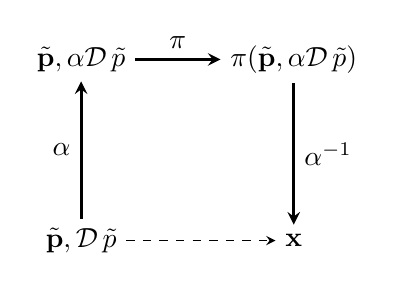
\begin{tikzpicture}
        % Define arrow style with larger heads
        \tikzset{->, arrow style/.style={draw=black, ->, >=stealth, line width=1.0pt}}
        \tikzset{->, arrow style 2/.style={draw=black, ->, >=stealth, line width=0.5pt, scale=2, dashed}}
    
        % Define the positions of the equations
        \node (A) at (0,0) {$\tilde{\mathbf{p}}, \mathcal{D\,} \tilde p$};
        \node (B) at (2.7,0) {$\mathbf{x}$};
        \node (C) at (2.7,2.3) {$\pi (\tilde{\mathbf{p}}, \alpha \mathcal{D\,} \tilde p)$};
        \node (D) at (0,2.3) {$\tilde{\mathbf{p}}, \alpha\mathcal{D\,} \tilde p$};
    
        % Draw the arrows and add the short equations
        \draw[arrow style] (C) -- (B) node[midway, right] {$\alpha^{-1}$};
        \draw[arrow style] (D) -- (C) node[midway, above] {$\pi$};
        \draw[arrow style] (A) -- (D) node[midway, left] {$\alpha$};
        \draw[arrow style 2] (A) -- (B) node[midway, above] {};
    \end{tikzpicture}
    % \vspace{.1\baselineskip}
    \caption{}
    \label{fig:diagram_iter}
\end{subfigure}
\begin{subfigure}[b]{0.23\textwidth}
    \captionsetup{justification=centering}
    \includegraphics[width=\textwidth,trim=0.2cm 0.5cm .2cm .0cm,clip]{figures/scale_factor_time_iter4.png}
    \caption{}
    \label{fig:plot_iter}
\end{subfigure}
\vspace{-.3\baselineskip}
\caption{Iterative traversal time adaptation: (a) Time scaling method preserves trajectory shape while reducing speed. (b) Iterative application finds optimal scaling factor $\alpha_{\text{goal}}$ to match target time.}
\vspace{-.6\baselineskip}
\end{figure}

\begin{figure}[h]
    \centering
    \includegraphics[width=0.45\textwidth,trim=0.2cm 0.5cm -0.2cm 0.2cm,clip]{figures/scale_factor_err.png}
    \caption{Tracking error depending on the scale factor. Shading indicates standard deviation.}
    \label{fig:scale_factor_err}
    \vspace{-1\baselineskip}
\end{figure}

The planning policy is trained to generate time allocations that minimize overall traversal time. 
Therefore, by verifying that the scale factor $\alpha_\text{goal}$ is greater than one, which indicates that the target arrival time exceeds the minimal traversal time, we can assess the feasibility of each initial A* path. 
Among the optimized trajectories, we select the one with the minimal and feasible traversal time using the following equations:
\begin{equation}
\begin{gathered}
\argmax_{k} \; \tilde{\mathbb{P}}(\tilde p_{\text{goal}}^k) - T_\text{goal}^k \\ 
\text{subject to}\;\; \alpha_\text{goal}^k \geq 1, \norm{p^k- q^k}_2 < \delta_\text{max} 
\label{eqn:homotopy_1}
\end{gathered}
\end{equation}
where $\tilde{\mathbb{P}}(\tilde p_{\text{goal}}^k)$ represents the likelihood obtained from the target position prediction model, normalized to $[0,1]$ within the batch of goal position candidates.
$p^k$ is the polynomial trajectory derived from waypoints $\tilde p$ towards the goal position $\tilde p_{\text{goal}}^k$ and time allocations determined by the planning policy.
$q^k$ is obtained by linearly interpolating the A* path. 
The L2 distance between $p^k$ and $q^k$ is calculated as the maximum distance between corresponding points sampled uniformly along both paths. 
By rejecting trajectories that deviate excessively from the A* path, we ensure collision avoidance for the final polynomial trajectory.
If no feasible trajectory is available, we select the one with the longest target time, allowing us to wait until a feasible path becomes available.

%  as follows:
% \begin{equation}
% \begin{gathered}
% \argmax_{k} \; \tilde{\mathbb{P}}(\tilde p_{\text{goal}}^k, T_\text{goal}^k) + T_\text{goal}^k \\ 
% \text{subject to}\;\; \alpha_\text{goal}^k < 1, \norm{p^k- q^k}_2 < \delta_\text{max} 
% \label{eqn:homotopy_2}
% \end{gathered}
% \end{equation}

\subsection{Target position prediction}
% The prediction model predicts $N_{pred}$ samples
We assess our algorithm using three distinct models for target position: 1) the target drone’s actual future trajectory (ground truth), 2) a noisy version of the ground truth, and 3) predictions based on a Gaussian mixture model (GMM).
The prediction model estimates the distribution of goal positions for target time $T_\text{goal}$, $\mathbb{P}(\tilde{p}_\text{goal})$.
\cref{fig:compare_pred} illustrates the three different prediction models used for evaluation.

\begin{figure}[]
    \centering
    % \captionsetup{justification=centering}
    \includegraphics[width=0.48\textwidth,trim=0.15cm 2.8cm 0.15cm 1.5cm,clip]{figures/target_predictions.png}
    \caption{Comparison of prediction models.}
    \label{fig:compare_pred}
    \vspace{-1\baselineskip}
\end{figure}

Initially, we evaluate our algorithm with the exact ground truth trajectory. 
We uniformly select a candidate target position at each $dt$ interval for $N_\text{pred}$ steps, starting from the current time step.
This results in target position candidates $\tilde{\mathbf{p}}_{\text{target}} =[\tilde p_{\text{target}, 1}, \dots, \tilde p_{\text{target}, N_\text{pred}}]$ which corresponds to the time steps, $T_\text{goal} \in [dt, 2dt, \dots, N_\text{pred}dt]$.

Next, we introduce Gaussian noise to simulate a noisy prediction environment. 
Along the $N_\text{pred}$ steps, we $N_\text{batch}$ positions around the ground truth for each step, resulting in a total of $N_\text{pred} \times N_\text{batch}$ position candidates.
The variance of this noise increases linearly with each prediction time step to reflect growing uncertainty as follows:
\begin{equation}
    \mathbb{P}(\tilde{\mathbf{p}}_{\text{goal}}) = \mathcal{N}(\tilde{\mathbf{p}}_{\text{goal}} | \tilde{\mathbf{p}}_{\text{target}}, \text{diag}([1 \cdots N_\text{pred}]) \sigma_{pred}^2)
\end{equation}

Lastly, to implement the full planning pipeline, we train a Gaussian mixture model to predict the target drone’s trajectory distribution, which is often used to predict the trajectory of vehicles or pedestrians~\cite{wiest2012probabilistic, wakulicz2023topological, salzmann2020trajectron}.
In the planning environment, we generate random minimum snap trajectories and subsample trace points along these paths. 
We use the sequences of non-colliding points to train the prediction model. 
The distribution of sampled reference positions $\tilde{\mathbf{p}} \in \mathbb{R}^{3 \times (N_\text{obs}+N_\text{pred})}$ is modeled with a mixture of Gaussian distributions:
\begin{equation}
    \mathbb{P}(\tilde{\mathbf{p}}) = \sum_{i=1}^{N_\text{GMM}} \pi_i \mathcal{N}(\tilde{\mathbf{p}}| \mathbf\mu_i, \mathbf\Sigma_i)
\end{equation}
The Gaussian mixture model is trained using the expectation maximization (EM) algorithm, which optimizes the weights and parameters of each Gaussian distribution. 
% During prediction, the distribution of the point sequences is marginalized based on the observed positions of the target drone to obtain the posterior distribution of its location. 
% Specifically, the distribution of future positions, $\tilde{\mathbf{p}}_{\text{goal}}$, is calculated by marginalizing the observed reference positions $\mathbf{p}_{\text{obs}} \in \mathbb{R}^{3 \times N_\text{obs}}$ from the distribution of reference positions $\tilde{\mathbf{p}}$. 
The future position distribution $\tilde{\mathbf{p}}_{\text{goal}}$ is obtained by marginalizing observed reference positions $\mathbf{p}_{\text{obs}} \in \mathbb{R}^{3 \times N_\text{obs}}$ from the reference position distribution $\tilde{\mathbf{p}}$, based on observed target drone positions.
Similarly to the noisy ground truth scenario, $N_\text{batch}$ positions are sampled at each of the $N_\text{pred}$ time steps, and any target positions that are unreachable or located on obstacles are rejected.

% \begin{equation}
%     \mathbb{P}(\mathbf{p}_{\text{f}} | \mathbf{p}_{\text{o}}) = \sum_{i=1}^{N_\text{GMM}} \pi_{i, \text{f}|\text{o}} \mathcal{N}(\mathbf{p}_{\text{f}} | \mathbf\mu_{i, \text{f}|\text{o}}, \mathbf\Sigma_{i, \text{f}|\text{o}})
% \end{equation}
